\documentclass[12pt,onecolumn]{article}


\usepackage{float}
\usepackage{mathtools}
\usepackage[russian]{babel}
\everymath{\displaystyle}

\usepackage[usenames]{color}
\usepackage{colortbl}

\usepackage{geometry}
\geometry{
  a4paper,
  top=15mm, 
  right=10mm, 
  bottom=15mm, 
  left=10mm
}

\begin{document}

\begin{center}
    Санкт-Петербургский Национальный Исследовательский\\ 
    Университет ИТМО\\
    Факультет Программной Инженерии и Компьютерной Техники\\
    % \includegraphics{itm.jpg}
\end{center}
\vspace{1cm}


\begin{center}
    \large \textbf{Вариант №3118100}\\
    \textbf{Лабораторная работа №2}\\
    по дисциплине\\
    \textbf{\textit{'Программирование'}}
\end{center}

\vspace{3cm}
\begin{flushright}
  Выполнил Студент  группы P3118: \\
  \textbf{Михеев Илья}\\
  Преподаватель: \\
  \textbf{Письмак Алексей Евгеьевич}\\
\end{flushright}

\vspace{14cm}
\begin{center}
    г. Санкт-Петербург\\
    2022г.
\end{center}

\newpage

\tableofcontents

\vspace{1cm}

\section{Текст задания}
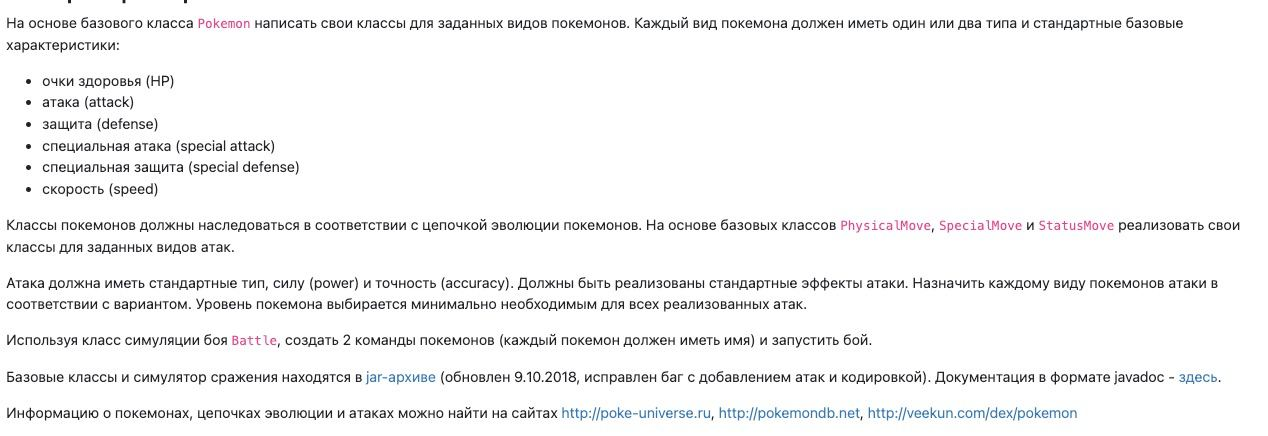
\includegraphics[width=\columnwidth]{imgs/lab2task.png}
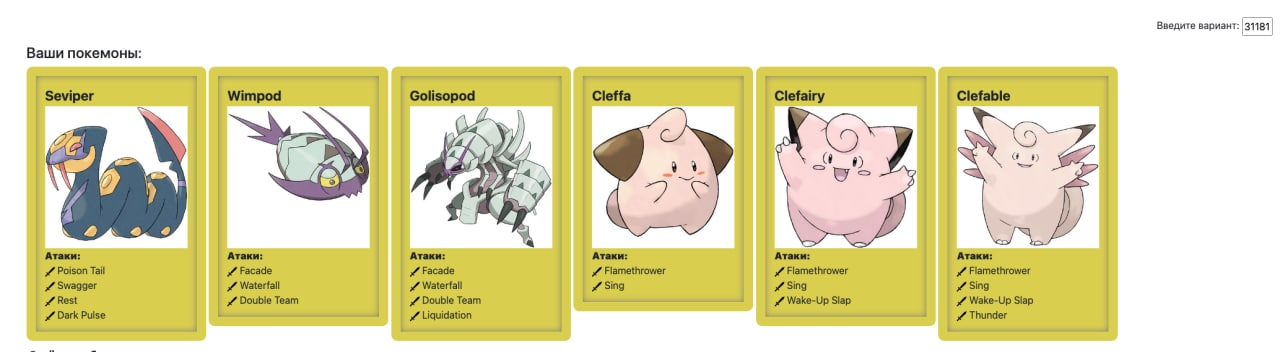
\includegraphics[width=\columnwidth]{imgs/lab2pokes.png}

\section{Диаграмма классов}
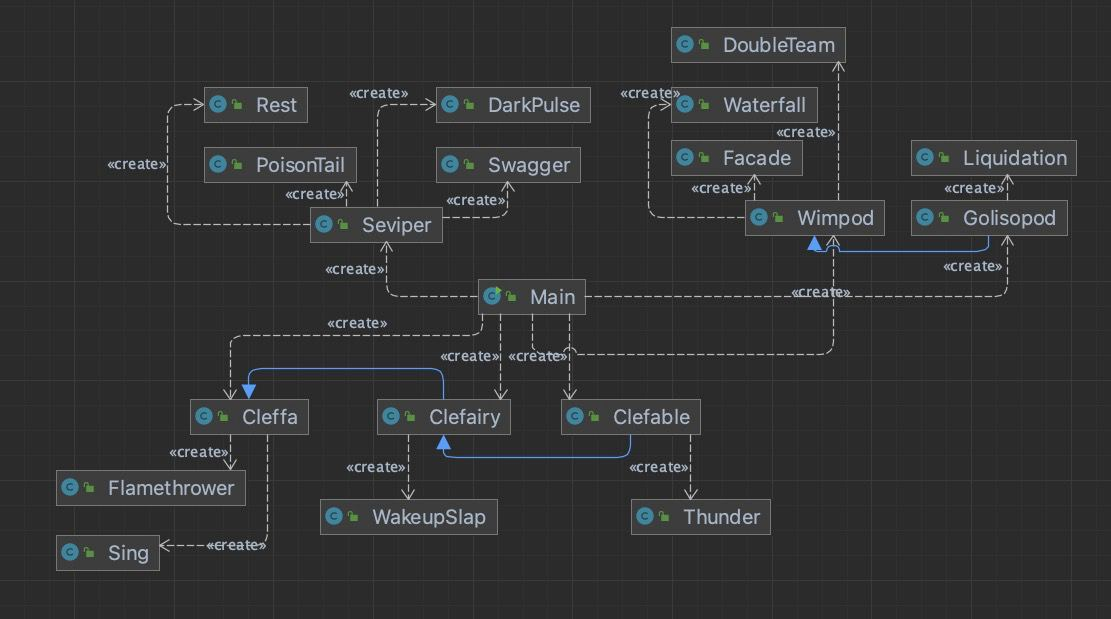
\includegraphics[width=\columnwidth]{imgs/lab2diagram.png}

\section{Исходный код программы}
https://github.com/Ne0Ment/ITMO-proga/blob/main/lab2/src/
\begin{center}
  
\includegraphics[width=7cm]{imgs/lab2qr.png}
\end{center}
\section{Результат выполнения}
Seviper ArLet из команды фиолетовых вступает в бой! \\
Cleffa Gepeusea из команды белых вступает в бой! \\
Seviper ArLet uses Swagger. \\
Cleffa Gepeusea уменьшает атак у. \\
\\
Cleffa Gepeusea uses Sing. \\
Seviper ArLet засыпает\\
\\
Cleffa Gepeusea растерянно попадает по себе.\\
Cleffa Gepeusea теряет 2147483647 здоровья.\\
Cleffa Gepeusea теряет сознание.\\
Clefairy Fergie из команды белых вступает в бой!\\
Clefairy Fergie uses Wake-up Slap.\\
Seviper ArLet теряет 2 здоровья.\\
\\
\\
Clefairy Fergie uses Wake-up Slap.\\
Seviper ArLet теряет 3 здоровья.\\
\\
\\
Seviper ArLet uses Swagger.\\
Clefairy Fergie уменьшает атаку.\\
\\
Clefairy Fergie uses Sing.\\
Seviper ArLet засыпает\\
\\
Seviper ArLet борется с соперником.\\
Clefairy Fergie теряет 5 здоровья.\\
Seviper ArLet теряет 1 здоровья.\\
\\
Clefairy Fergie uses Wake-up Slap.\\
Seviper ArLet восстанавливает 1 здоровья.\\
\\
Seviper ArLet uses Poison Tail.\\
Clefairy Fergie теряет 17 здоровья.\\
Clefairy Fergie теряет сознание.\\
Clefable Slonser из команды белых вступает в бой!\\
Seviper ArLet промахивается\\
\\
Clefable Slonser uses Sing.\\
Seviper ArLet засыпает\\
\\
Clefable Slonser uses Thunder.\\
Seviper ArLet теряет 4 здоровья.\\
Seviper ArLet парализован\\
\\
\\
Seviper ArLet промахивается\\
\\
Clefable Slonser uses Flamethrower.\\
Seviper ArLet теряет 4 здоровья.\\
Seviper ArLet теряет сознание.\\
Wimpod ExcaLet из команды фиолетовых вступает в бой!\\
Wimpod ExcaLet борется с соперником.\\
Clefable Slonser теряет 4 здоровья.\\
Wimpod ExcaLet теряет 1 здоровья.\\
\\
Clefable Slonser uses Sing.\\
Wimpod ExcaLet засыпает\\
\\
Clefable Slonser uses Sing.\\
\\
\\
Clefable Slonser uses Thunder.\\
Wimpod ExcaLet теряет 12 здоровья.\\
Wimpod ExcaLet теряет сознание.\\
Golisopod NeoLet из команды фиолетовых вступает в бой!\\
Clefable Slonser uses Flamethrower.\\
Golisopod NeoLet теряет 5 здоровья.\\
\\
Golisopod NeoLet промахивается\\
\\
Clefable Slonser uses Thunder.\\
Golisopod NeoLet теряет 12 здоровья.\\
Golisopod NeoLet теряет сознание.\\
В команде фиолетовых не осталось покемонов.\\
Команда белых побеждает в этом бою!\\

\section{Вывод}
Во время выполнения лабораторной работы я узнал основные принципы ООП а также закрепил их используя язык Java.

\end{document}